\chapter{Cluster distortion and bipolaron formation}
\label{chap:ground}

As discussed in section \ref{sec:lattice-distortions}, from the ground state of the model hamiltonian (\ref{eq:full-hamiltonian}) we can calculate, using (\ref{eq:dvsuir}), the difference in bond distances in the CuO$_2$ cluster for different values of the coupling parameter $\lambda_{ir}$.
First, in section \ref{sec:grd-phonon-proj} of this chapter, we reproduce the previous work by Mustre de Le\'{o}n \textit{et al.} \cite{MustredeLeon1992} which, from a similar calculation, determined that the relevant couplings are in the intermediate regime. Furthermore we present a more detailed analysis of the dependende of this cluster distortion with the coupling $\lambda_{ir}$ and show that it is dynamical only in a narrow coupling range.

Subsequently we turn our attention to the bipolaron binding energy. 
We can identify the difference between the ground state energy in the absence of electron-lattice interaction ($\lambda_{ir}=0$) and its value for the coupling value where this polaronic behaviour sets in as the bipolaron binding enerygy.
In section \ref{sec:grd-binding-energy} we calculate this binding energy comparing it with experimental results.
We also calculate the isotopic shift, as defined in (\ref{eq:isot-shift-def-grd}), for the oxygen substitution$^{16}$O$\rightarrow ^{18}$O as a function of $\lambda_{ir}$.

\section{Cu(1)-O(4) local distortion}
\label{sec:grd-phonon-proj}

The wavefunction projection into phonon coordinates (\ref{eq:phonon-coord-projection}) gives information about the coodinates of the three atoms in the CuO$_2$ cluster.
In particular, the phonon coordinate\footnote{The phonon coordinates are  defined in (\ref{eq:uR}, \ref{eq:uir}).} $u_{ir}$ is directly proportional to the distance distortion in the CuO$_2$ cluster, $d$, as shown in (\ref{eq:dvsuir}).
Figure \ref{fig:ph-ground} shows the ground state projected into phonon coordinates $(u_R,u_{ir})$ for three representative electron-lattice coupling values $\lambda_{ir}=0, 0.13$ and 0.25 eV.
The projection along $u_R$ is harmonic in all cases.
From the $\lambda_{ir}=0$ case the wavefunction's projection has a maximum at $u_{ir}=0$ impliying, as expected, there is no distortion in the cluster.
In the middle coupling regime, exemplified in Fig. \ref{fig:ph-ground} by $\lambda_{ir}=0.13$ eV, there are clearly two peaks present although they are not fully separated.
Since the probability amplitude is not neglible between the two maxima the system can \textit{tunnel} between both possible configurations with the longer distance in the first oxygen or the second bond.
This observation can be interpreted as a dynamic distortion in the cluster that can only be experimentally identifyied with a technique with a similar timescale (see discussion in secion \ref{sec:dynamic_dist}). 
For greater coupling values the two peaks are completely separated and the distortion becomes static.

\begin{figure}[ht!]
  \centering
  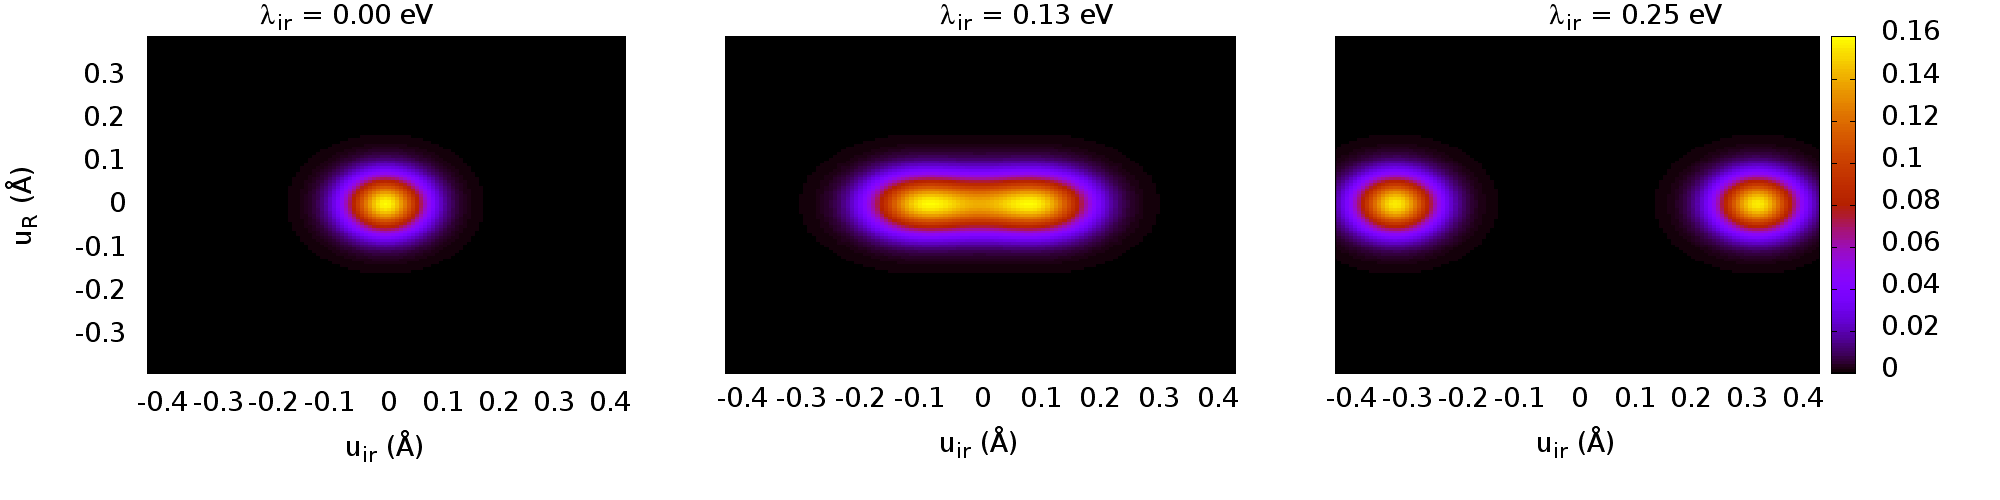
\includegraphics[width=1.0\textwidth]{images/ph-ground.png}
  \caption{Ground state's projection into phonon coordinates for three different values of the coupling parameter $\lambda_{ir}$.}
  \label{fig:ph-ground}
\end{figure}

Since the projection into $u_R$ does not change, giving that we are considering only $\lambda_R=0$, we calculated the projections with $u_R=0$ with variable $u_{ir}$ for different coupling values.
The left panel of figure \ref{fig:uir-vs-coupl} shows a plot of this comparison.
From here we can see that the distortion only sets in for $\lambda_{ir}$ greater than $\sim 0.12$ eV and becomes static (the two peaks are fully separated) for $\lambda_{ir}$ greater that $\sim 0.16$ eV.
In the right panel of figure \ref{fig:uir-vs-coupl} we show the cluster distortion $d$ calculated from the maxima of the previous projection.
Here we can see that the observed cluster distortion of $\sim 0.13$ \AA\ \cite{MustredeLeon1990} is reproduced in the intermedite coupling values. 
In particular, $\lambda_{ir}=0.1263$ eV reproduces that distortion.
From this plots we observe that it is only in the narrow range  $\sim 0.12 < \lambda_{ir} < \sim 0.16$ that a dynamical cluster distortion is present. 

\begin{figure}[ht!]
  \centering
  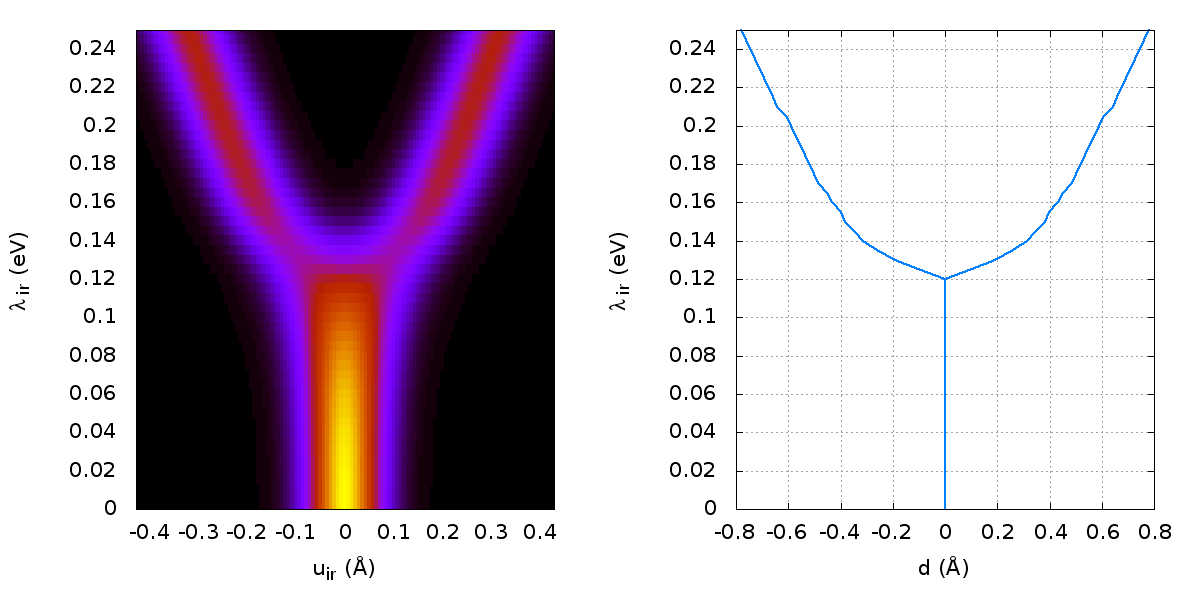
\includegraphics[width=1.0\textwidth]{images/uir-vs-coupl-d.png}
  \caption{Projection into phonon coordinates with $u_R=0$ (left panel) and calculated cluster distortion $d$ (right panel) for different $\lambda_{ir}$ coupling values.}
  \label{fig:uir-vs-coupl}
\end{figure}

\section{Bipolaron binding energy}
\label{sec:grd-binding-energy}

The bipolaron formation energy is $E_p = E(\lambda_{ir}=0)- E(\lambda_{ir}=0.13$ eV$) \sim 42$ meV and corresponds to the bipolaron binding energy. 
This value compares favorably with the value obtained from femtosecond time-domain spectroscopy ($E_p \sim 45$ meV for YBa$_2$Cu$_3$O$_7$ \cite{Demsar1999}. 
We also find that if we consider a smaller electron-lattice coupling such that the distortion is 0.08 $\AA$, as that observed for in plane Cu(2)-O in La$_{1.85}$Sr$_{0.15}$CuO$_4$ \cite{Bianconi1996}, we obtain $E_p \sim 32$ meV, which is also comparable to estimates for the pseudogap formation energy in this system \cite{Kusar2005}.

\section{Isotopic effects in bipolaron formation}
\label{sec:grd-isotopic}

For the ground state we define the energy isotopic shift $\Delta_g$ in a similar way but with the energies measured relative to the uncoupled system (that is, the system with $\lambda_{ir}=\lambda_R=0$) (see \ref{eq:isot-shift-def-grd}):

\begin{equation}
  \Delta_g = \frac{\Delta E_g(^{16}O)- \Delta E_g(^{18}O)}{\Delta E_g(^{16}O)} \times 100 
\end{equation}

where $\Delta E_g \equiv E_g - E_g(\lambda_{ir}=0, \lambda_R=0)$.\footnote{To calculate this energies we need to take into account the \textit{zero-point energy} in the phononic part $H_{ph}$ from (\ref{eq:full-hamiltonian}) which is not explicitly included in previous publications.}

The following figure plots this isotopic shift:

\begin{figure}[ht!]
  \centering
  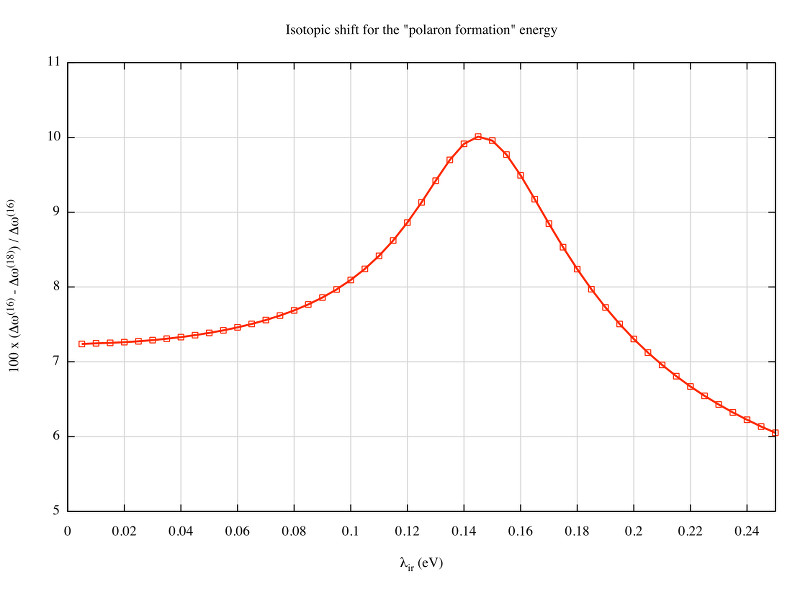
\includegraphics[width=0.8\textwidth]{images/isot_polaron_formation.jpg}
  \caption{Isotopic shift of the polaron formation energy.}
  \label{fig:isot_polaron_formation}
\end{figure}

Although $\Delta_g$ doesn't change sign, as the isotopic shift of the polaron tunneling state, it shows a maximum in the middle coupling regime reminiscent of the maximums, minimums or inflection points in the isotopic shifts for all the other excitations.